\section{2D coordination algorithms}

\subsection{Nearest frontier approach}
\begin{frame}
     \frametitle{Nearest frontier approach}
     \begin{itemize}
     	\item[-] Choose the nearest frontier region to explore
%     	\item[-] Yamauchi's technique consists in selecting the shortest path to the nearest frontier. 
     	\item[-] The target cell:
     	\begin{equation}
     	t_{NF} = \argmin_{a \in F} L(a)
     	\label{equation:t-nf}
     	\end{equation}	
     	\item[-] “Given what you know about the world, where should you move to gain as much new	information as possible?”\footcite{Yamauchi1998} 
     	\item[-] Extension to multiple robots
     \end{itemize}
     
\end{frame}

\subsection{Cost-utility approach}
\begin{frame}
	\frametitle{Cost-utility approach}
	\begin{itemize}
		\item[-] Next-Best-View\footcite{GonzlezBaos2002} 
		\item[-] The benefit $B_{CU}(a)$ to reach a candidate cell $a$:
		\begin{equation}
		B_{CU}(a) = U(a) - \lambda_{CU}C(a)
		\label{equation:cost-utility}
		\end{equation}
%		\begin{equation}
%		U(a) = \frac{U_{nex}(a, R_{s})}{\pi R_{s}^{2}}
%		\end{equation}
%		\begin{equation}
%		C(a) = \frac{L(a)}{max_{b \in F}L(b)}
%		\end{equation}
		\item[-] The target cell $t_{CU}$:
		\begin{equation}
		t_{CU} = \argmax_{a \in F} B_{CU}(a)
		\end{equation}
		\item[-] Coordination by reducing the utility of a frontier point\footcite{Burgard2000}
		\item[-] Optimized using the Hungarian method\footcite{Burgard2005}
	\end{itemize}
	
\end{frame}

\subsection{Market-based approach}
\begin{frame}
	\frametitle{Market-based approach}
%	\begin{figure}
%		\centering
%		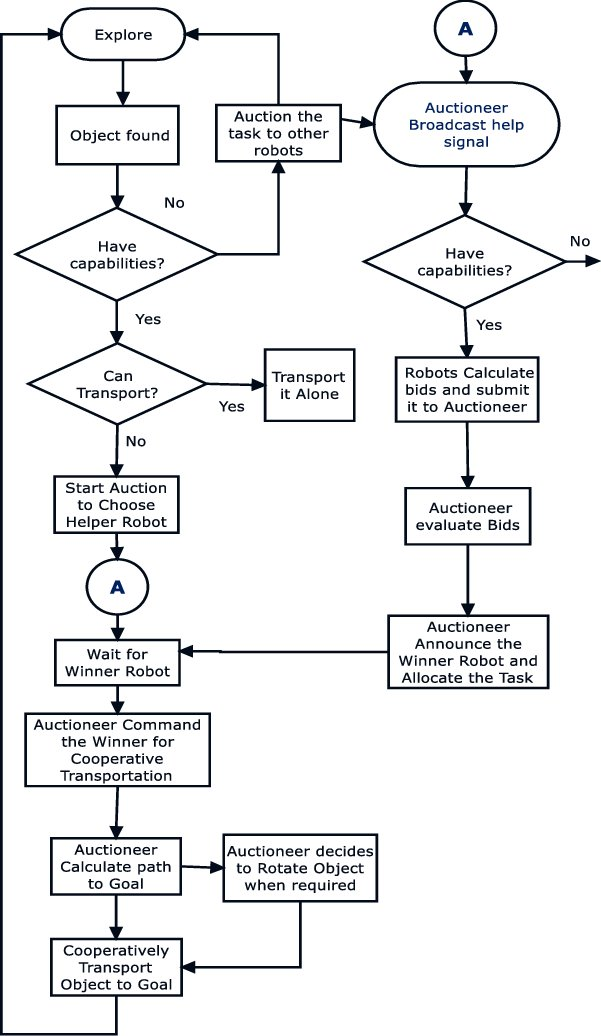
\includegraphics[height=6cm, width=5cm]{figures/auction}
%%		\caption{Auction}
%	\end{figure}
	\begin{itemize}
		\item[-] Introduced by Zlot\footcite{Zlot2002}
		\item[-] Robots as \textbf{sellers} and \textbf{buyers}
%		\item[-] %After reaching a current goal point,
		\item[-] A robot initiates an \textbf{auction}
		\item[-] Each buyer $i$ submits a bid of:
		\begin{equation}
			B_{i} = P_{r} + \alpha(v_{i} - P_{r})
		\end{equation}
%		Next, the robot tries
%		to sell each of its tasks to all robots with which it is currently able to communicate, via an auction. The other
%		robots each submit bids, which encapsulate their cost
%		and revenue calculations. The robot offering the task
%		(the auctioneer) waits until all robots have bid (up to a
%		specified amount of time). If any robot bids more than
%		the minimum price set by the auctioneer, the highest
%		bidder is awarded the task in exchange for the price of
%		the bid. Once all of a robot’s auctions close (all goals
%		on the robot’s tour have been sequentially offered),
%		that robot begins its tour by navigating towards its
		\item[-] The highest bidder is awarded 		
%		\item[-] For each point in auction, each robot makes a bid with its current profit aiming to minimize own travel distance and maximize new area information
%		not	dependent the central agent
		\item[-] Market model with limited communication range \footcite{Sheng2006} $\,$ \footcite{Michael2008}
		
%		W. Sheng, Q. Yang,
%		S. Ci and N. Xi [7] are proposed another, frontier based, distributed bidding model for
%		coordination of multiple robots. Besides, they consider the limited communication
%		environment in two ways. Firstly, they guided robots to stay close to each other by
%		considering the distances between robots in the coordination algorithm. Additionally,
%		they developed a new coding mechanism for map representation. New coding mechanism
%		reduced the exchanged data volume.
%Michael et al. [35] proposed a marked-based coordi-nation protocol where robots are able to bid for taskassignment with the assumption that every robot hasknowledge of the maximum number of robots that anygiven task can accommodate. Each auction is performedamong neighboring groups of robots and requires onlylocal communication.
%		
		\end{itemize}
	
\end{frame}

\subsection{Distributed approach}
\begin{frame}
	\frametitle{Distributed approach}
	\begin{itemize}
		\item[-] Assigning weights to frontier regarding to battery energy\footcite{Benkrid2017}
		\item[-] A scene partitioning scheme\footcite{LopezPerez2018}
	
%		Lopez-Perez et al. \cite{LopezPerez2018} proposed a new method to explore unknown areas by using a scene partitioning scheme and assigning weights to the frontiers between explored and unknown areas. Authors presented a distributed algorithm, which reduces the number of communications between robots as well as the time needed to explore unknown regions and the distance traveled by each robot. Algorithm implemented by Benkrid and Achour \cite{Benkrid2017} also assigns weights to frontier cells, but, on the other hand, depends on the energy of the battery of each robot.
%		
		\item[-] A team of $n$ mobile robots  \(\text{$\mathcal {R}$}\) = $ \{ 1, 2,..., N\}$
		\item[-] Every robot $i$ gets the list of frontier points  \(\text{$\mathcal {Y}$}\) = $ \{ 1, 2,..., M\}$
	\end{itemize}
%	The exploration is performed by, where the mobile robots do not have prior knowledge about the environment, i.e., the position of the boundaries and obstacles.  
	
	\begin{figure}
		\centering
		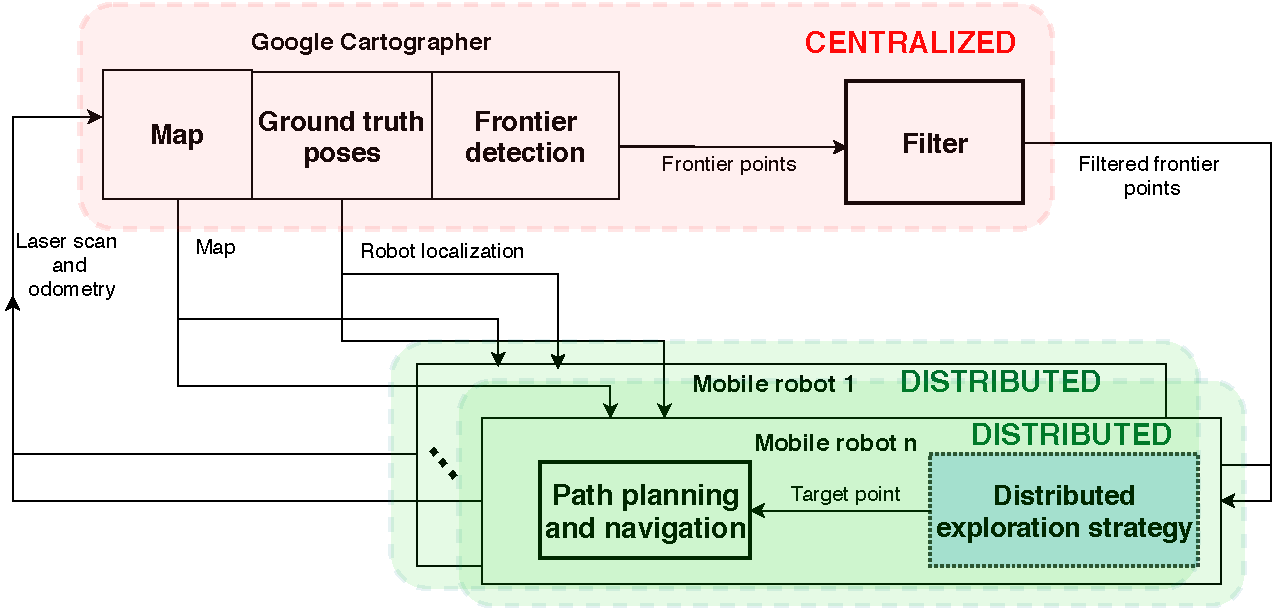
\includegraphics[width=0.6\textwidth]{figures/diagram_exploration}
	\end{figure}
\end{frame}

\begin{frame}
	\frametitle{Distributed exploration strategy}
		\begin{columns}
			\begin{column}{0.5\textwidth}
				\begin{itemize}
					\item[-] Information exchanged: robot positions and current robot target point 
					\item[-]  \textit{Weight function}: 
					\begin{equation}
					{W}_{ij}= {C_{ij}} - {U_{j}} + {F_{ij}}
					\label{weight}
					\end{equation}
					\item[-] \textbf{Event-based} target point assignment process  
				\end{itemize}
			\end{column}
			\begin{column}{0.5\textwidth}  %%<--- here
				\begin{center}
					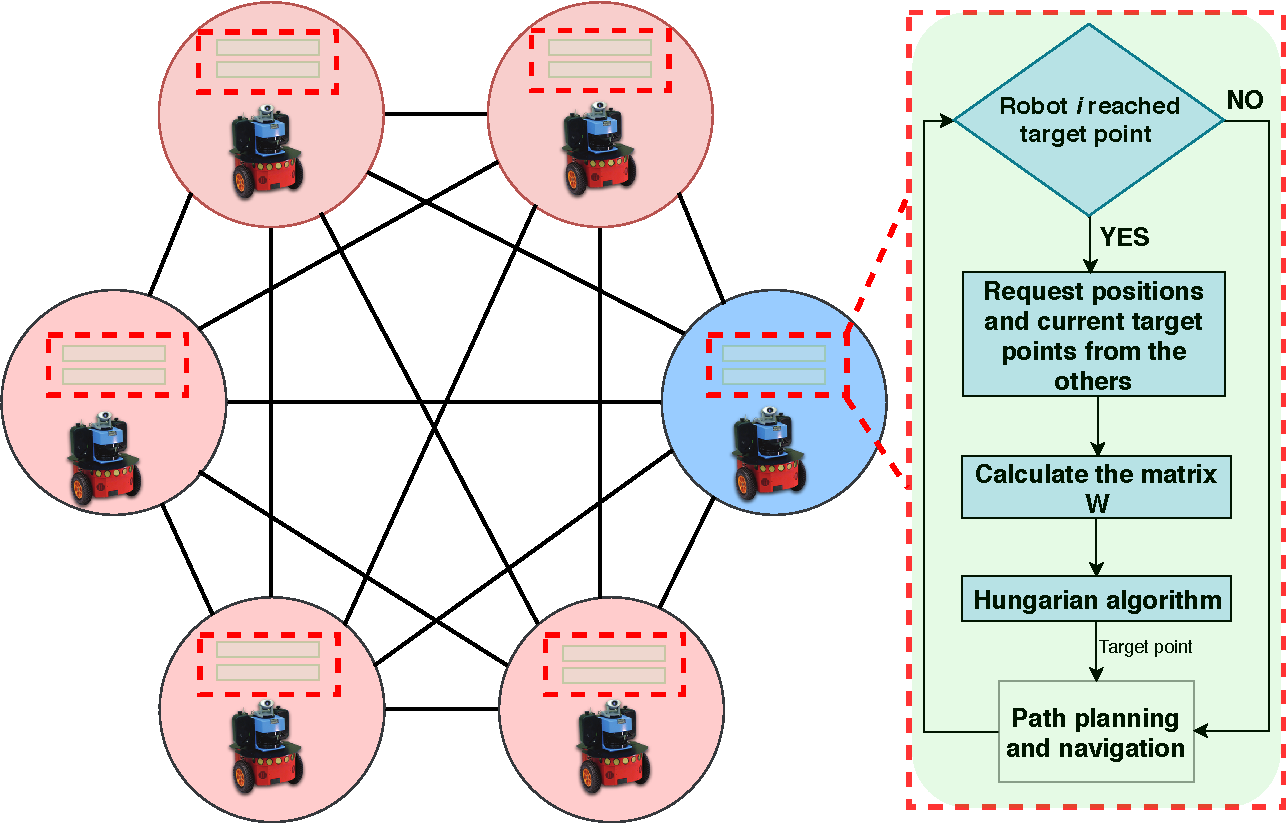
\includegraphics[width=1\textwidth]{figures/struktura_vol3}
					\label{fig:gauss}
				\end{center}
			\end{column}
		\end{columns}	
\end{frame}

\begin{frame}
	\frametitle{Distributed exploration strategy - simulation setup (1)}
	\begin{itemize}
		\item[-] Stage 2D simulator
		\item[-] Belgioioso Castle\footcite{fr_dataset} $\approx$ 225$m^{2}$
		\item[-] 2, 3 and 5 Pioneer P3-DX mobile robots
		\item[-] Average of 10 runs 
		\item[-] Compared with the Burgard's coordinated strategy
		\item[-] \textit{Coverage Ratio (CR)}:  \( \frac{\text{explored cells} \cdot 100}{\text{accessible cells}} \)
%The comparison of the coordinated and our decentralized strategy is shown using the \textit{Coverage Ratio (CR)} indicator which shows the percentage of the accessible terrain covered by the mobile robot team. It is calculated as:  \( \frac{\text{explored cells} \cdot 100}{\text{accessible cells}} \), 
	\end{itemize}
%	Simulations  were  carried  out  using  the  Stage  2D  simulator(Vaughan et al. (2012)), which simulates robot movement andlidar perception inside a loaded environment map. The ROSNavigation stack is used to control and direct the mobile robotstowards exploration goals.The scenario used in the simulation is the Belgioioso Castle,available  in  Haehnel  (2014)  and  shown  in  Fig.  5.  It  is  achallenging and a typical office-like scenario with a free spacearea of approximately 225m2. For the simulation, we use amodel of Pioneer P3-DX with maximum speed of 1.3 m/s, laserrange 20 m and 360◦laser scan window.The  algorithms  were  tested  with  teams  of  two,  three  andfive mobile robots
	\begin{figure}
		\centering
		
\includegraphics[width=0.6\textwidth]{figures/map}
	\end{figure}
\end{frame}

\begin{frame}
	\frametitle{Distributed exploration strategy - simulation setup (2)}
		\centering
		\href{presentation_video.mp4}{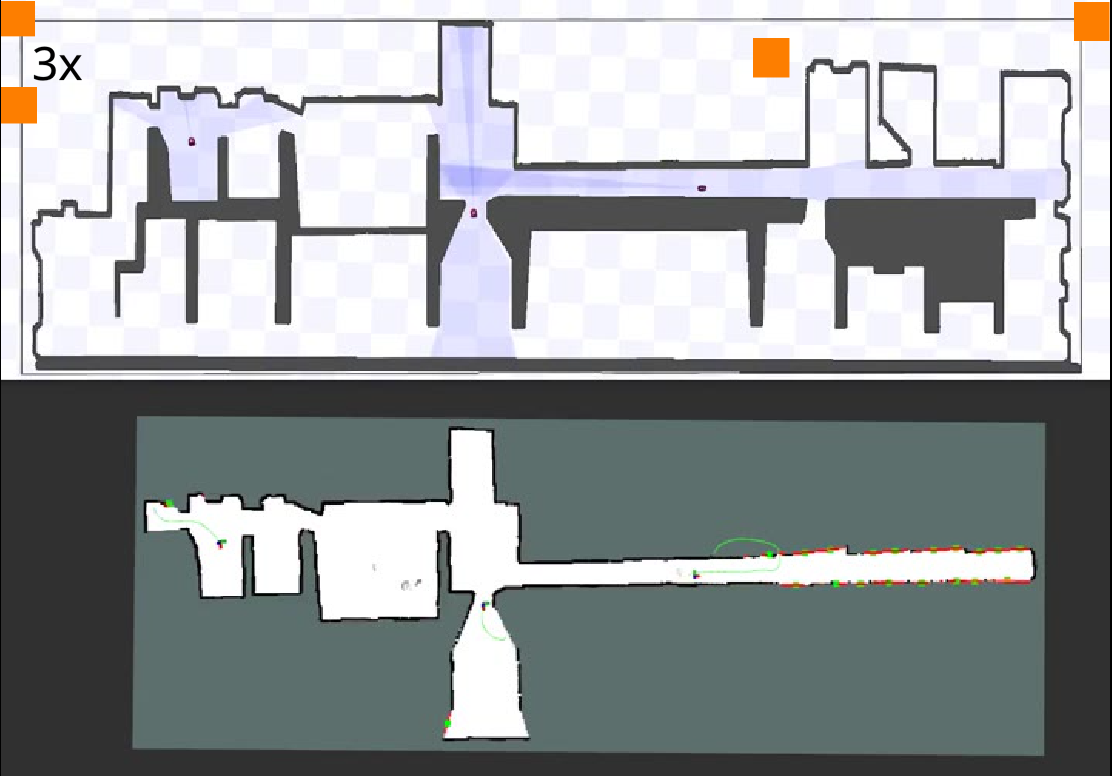
\includegraphics[width=0.8\textwidth]{figures/title_screen.png}}
\end{frame}

\begin{frame}
	\frametitle{Distributed exploration strategy - simulation results}
	\begin{figure}
		\centering
		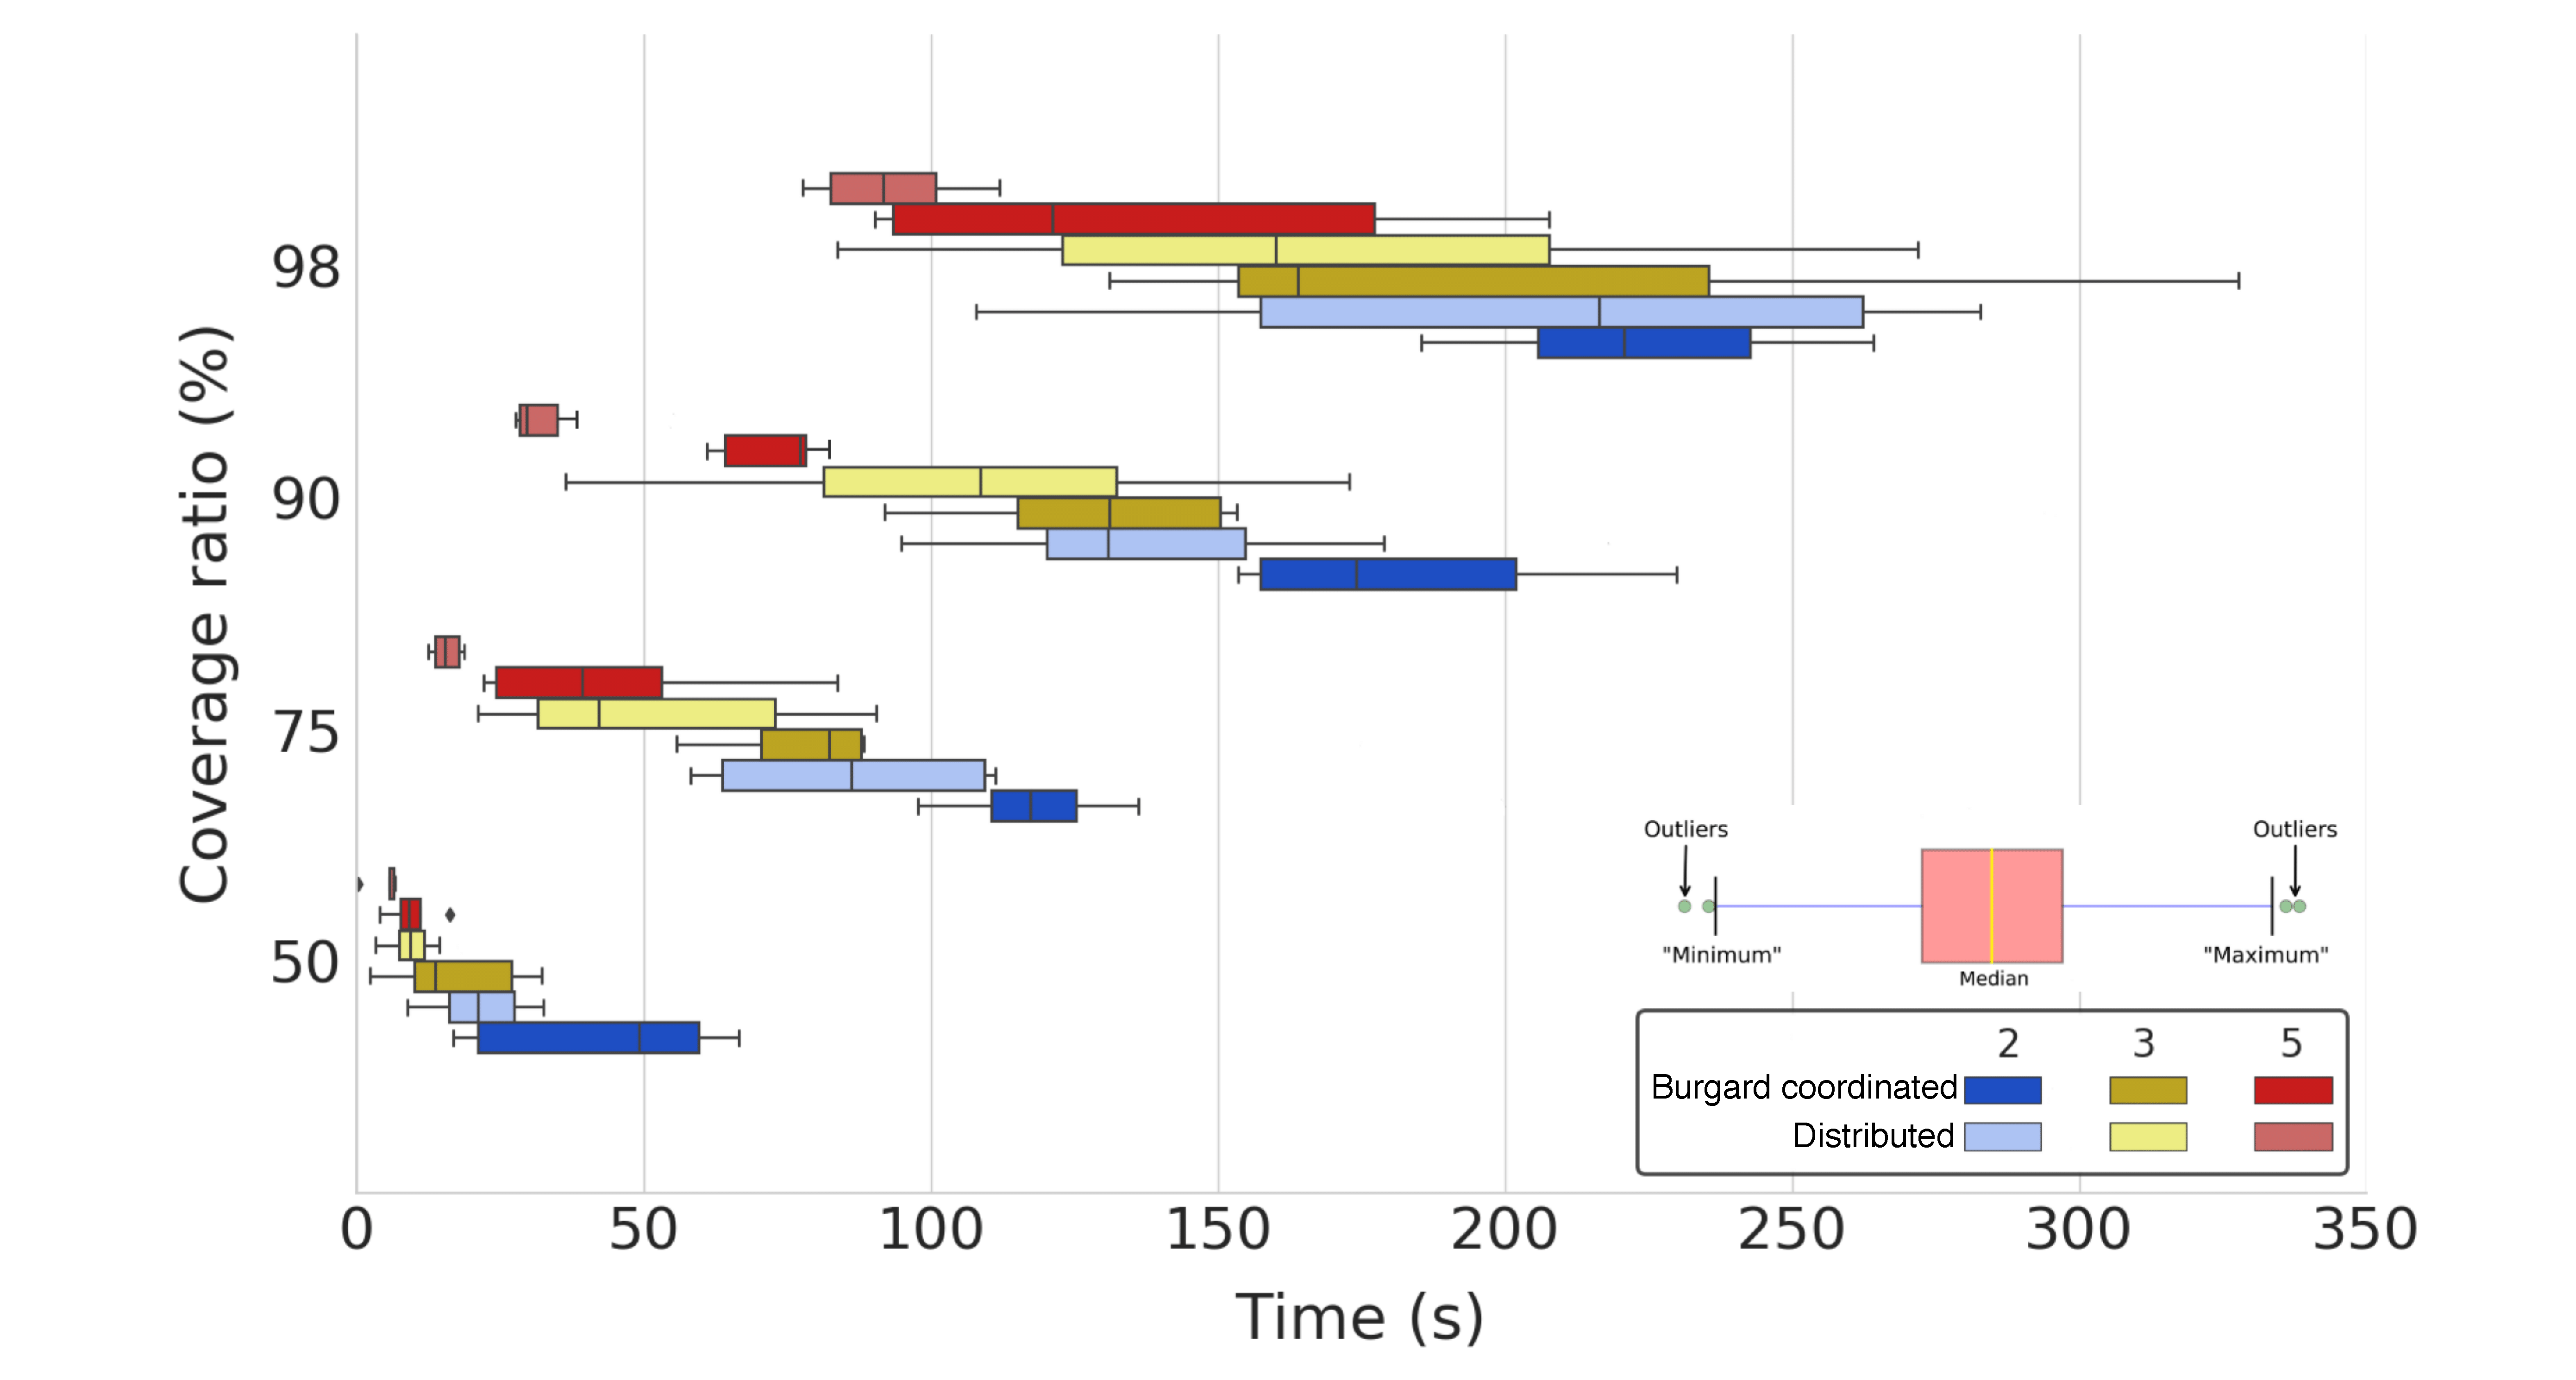
\includegraphics[width=0.9\textwidth]{figures/results_final}
	\end{figure}
	\begin{itemize}
		\item[-] To appear in IFAC 2020
	\end{itemize}
	
\end{frame}


